\chapter{CERN, the LHC and LHCb}
\label{CERN_LHC_LHCb}

The European Organisation for Nuclear Research (CERN) was founded in 1954 and began with 12 member states as a organisation to encourage European collaboration and the study of nuclear physics. Since it's foundation the collaborative nature of CERN allowed for large-scale expensive experiments and machines to be built. The Proton Synchrotron was CERN's flagship accelerator, operational in 1959 it had a circumference of 628~m and accelerated protons to 25 \gev, the highest energy at that time. Now 62 years since it's foundation CERN has grown to include 21 member states \footnote{about the other types of countries involved.} and is still at the forefront of high energy physics research. CERN’s latest accelerator, the Large Hadron Collider (LHC), is most energetic particle accelerator ever built, with a 27~km circumference the LHC was designed to protons at 14 \tev. This chapter shall discuss the LHC and the LHC beauty experiment, one of the experiments that uses collisions provided by the LHC.

\section{The LHC}
\label{LHC}


The LHC is a proton synchrotron that was designed to accelerate and collide two beams of protons travelling in oposite directions up to a center-of-mass energy of 14 \tev. Although operation of the LHC began in 2010 it is yet to reach design energy. The purpose of the LHC is to provide high energy proton collisions, the products of which are used for precision tests of the Standard Model (SM) and to search for new physics particles that go beyond the scope of the SM. There are four interaction points on the LHC ring where the beams are brought to collide, at these points various experiments detect and study the products of these collisions. The LHC can also accelerate lead-nuclei up to an energy of 2.76 \tev per nucleon, but it is only the products from proton collisions that are the topic of this thesis.


The protons for the LHC originate from hydrogen atoms in a gas, the gas is ionised to strip away the electrons and the protons are accelerated through a chain of particle accelerators of increasing energy before being injected into the LHC. The chain of accelerators, shown in Fig.~\ref{fig:accelerator_chain}, consists of existing accelerators that have been used in various experiments through the second half of the last century and have been upgraded to meet the requirements for providing protons for the LHC. 
The protons leave the chain of accelerators with of energy of 450 \gev per proton and in bunches of >~$10^{11}$, as the bunches injected into the LHC they are split into two oppositely circulating beams.
The LHC accelerates the protons to the desired center of mass energy using supercooled radio frequency cavities for acceleration and superconducting dipole magnets to bend the beams around the ring. 
The design configuration for the beams is to have 2808 bunches per circulating beam with 25 ns between each bunch, the bunches are focused using quadrupole magnets before being brought to collide at 4 interaction points with a bunch crossing rate of 40 MHz. 


\begin{figure}[htbp!] 
  \centering    
  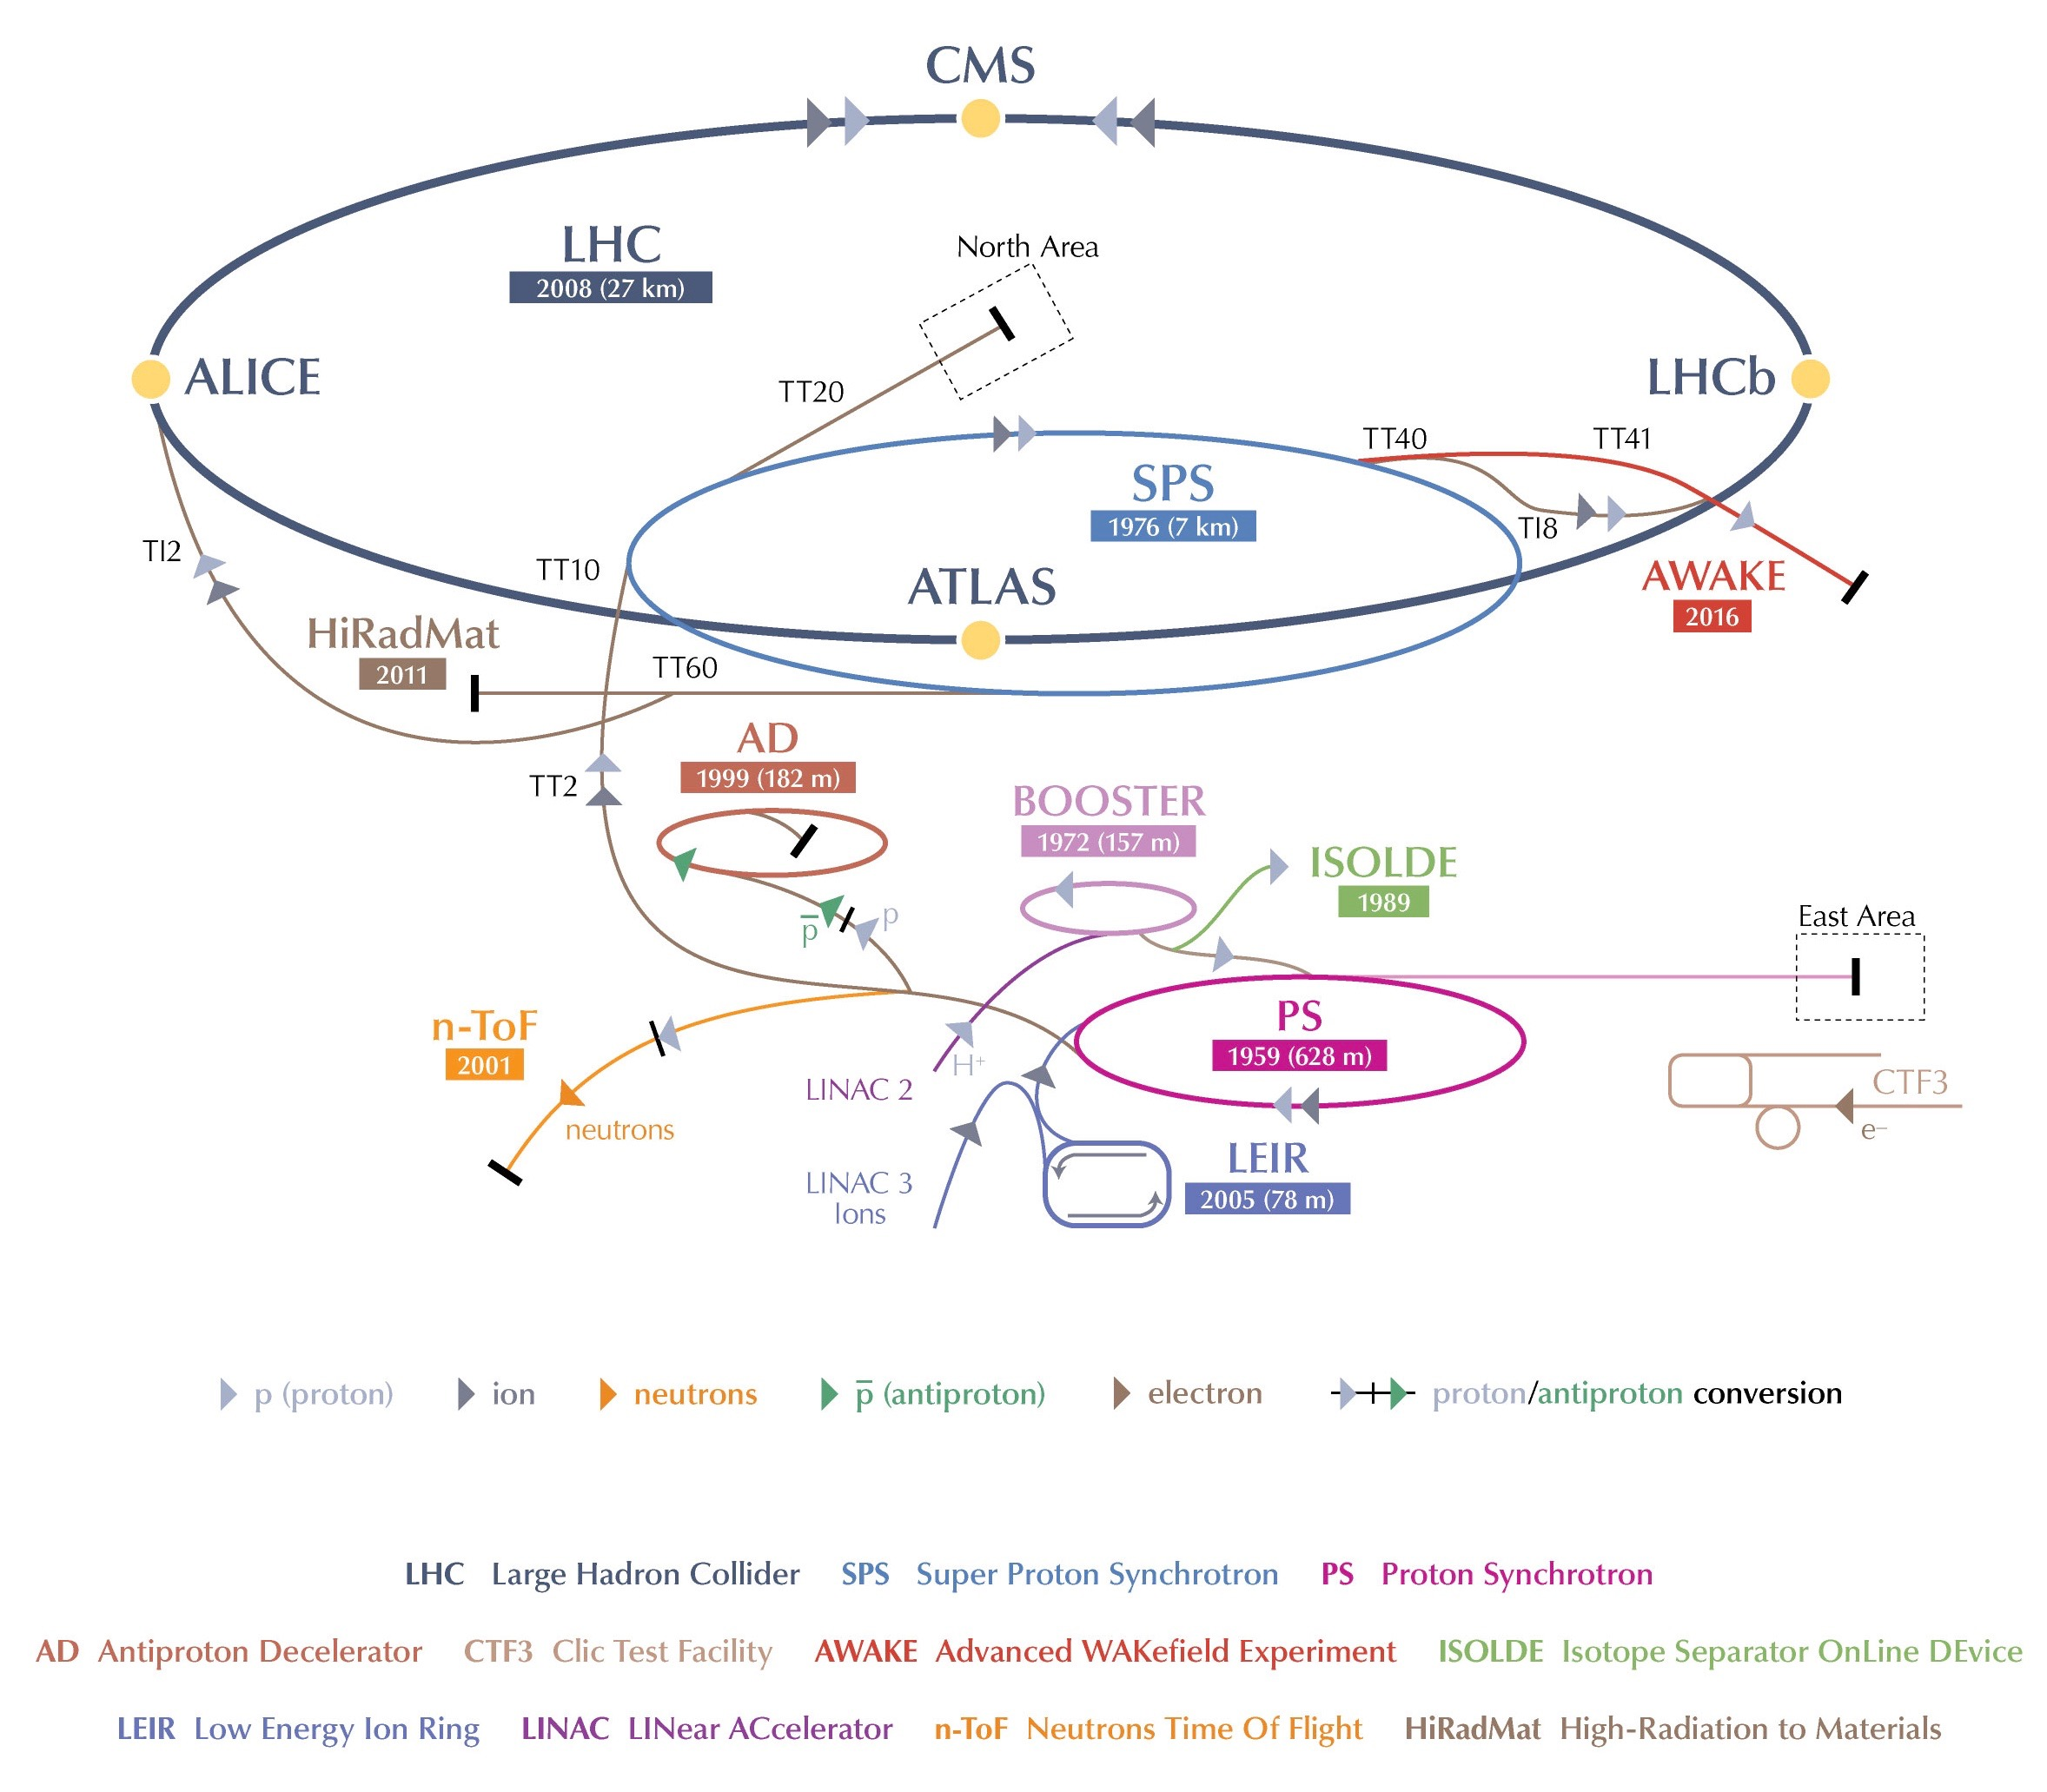
\includegraphics[trim = 125mm 2mm 125mm 90mm, clip, width=1.0\textwidth]{accelerator_complex.jpg}
  \caption{The accelerator complex at CERN. The chain of accelerators used to inject protons into the LHC consists of the Linac 2 accelerating protons to 50 \mev, the Proton Synchrotron Booster accelerating protons to 1.4 \gev, the Proton Synchrotron accelerating protons to 25 \gev and creating the desired spacing between proton bunches then finally the Super Proton Synchrotron accelerating protons to 450 \gev. Source: CERN.}
  \label{fig:accelerator_chain}
\end{figure}
